\documentclass[UTF8]{article}
\usepackage{graphicx}
\usepackage{subfigure}
\usepackage{amsmath}
\usepackage{makecell}
\usepackage[utf8]{inputenc}
\usepackage[space]{ctex} %中文包
\usepackage{listings} %放代码
\usepackage{xcolor} %代码着色宏包
\usepackage{CJK} %显示中文宏包
\usepackage{float}

\definecolor{mygreen}{rgb}{0,0.6,0}
\definecolor{mygray}{rgb}{0.5,0.5,0.5}
\definecolor{mymauve}{rgb}{0.58,0,0.82}
\lstset{
	backgroundcolor=\color{white}, 
	%\tiny < \scriptsize < \footnotesize < \small < \normalsize
	basicstyle = \scriptsize,       
	breakatwhitespace = false,        
	breaklines = true,                 
	captionpos = b,                    
	commentstyle = \color{mygreen}\bfseries,
	extendedchars = false,
	frame = shadowbox, 
	framerule=0.5pt,
	keepspaces=true,
	keywordstyle=\color{blue}\bfseries, % keyword style
	language = C++,                     % the language of code
	otherkeywords={string}, 
	numbers=left, 
	numbersep=5pt,
	numberstyle=\tiny\color{mygray},
	rulecolor=\color{black},         
	showspaces=false,  
	showstringspaces=false, 
	showtabs=false,    
	stepnumber=1,         
	stringstyle=\color{mymauve},        % string literal style
	tabsize=4,          
	title=\lstname           
}


%画图包
\usepackage{tikz}
%画图背景包
\usetikzlibrary{backgrounds}

%自定义命令
\newcommand{\psiG}{\psi_{G}}
%在tikz中画一个顶点
%#1:node名称
%#2:位置
%#3:标签
\newcommand{\newVertex}[3]{\node[circle, draw=black, line width=1pt, scale=0.8] (#1) at #2{#3}}
%在tikz中画一条边
\newcommand{\newEdge}[2]{\draw [black,very thick](#1)--(#2)}
%在tikz中放一个标签
%#1:名称
%#2:位置
%#3:标签内容
\newcommand{\newLabel}[3]{\node[line width=1pt] (#1) at #2{#3}}
\newcommand{\jumpLine} {\hspace*{\fill} \\}
\newcommand{\keypoint}[1]{$\bullet$\textbf{#1}\par}


\title{中国科学技术大学计算机学院\\《数据结构》报告}
\author{}
\date{}

\begin{document}
\maketitle
	\begin{figure}[H]
		\centering
		
\includegraphics[width=2.5in]{xiaohui.jpg}\vspace{0.5cm}\\
		\large{
			实验题目:图及其应用\\
			学生姓名:王章瀚\\
			学生学号:PB18111697\\
			完成日期:\today\\
		}\vspace{2cm}
		
		\large{计算机实验教学中心制\\2019年09月\\}
		\thispagestyle{empty}
		\clearpage  % 清除当页页码
	\end{figure}
	\newpage
	
	\section{实验要求}
	本次实验分为四个小实验。分别为\par
	\keypoint{寻找关节点}
	\keypoint{寻找最短路径}
	\keypoint{无向图的可视化}
	\keypoint{无向图中的最长圈}
	其中,无向图的可视化较为简单,只需要输出对应Graphviz的代码,故不多加阐述,只展示代码和效果。
	下面逐一进行分析。\par
	
	\subsection{寻找关节点}
	\subsubsection{概述}
	参考教材P177-178,算法7.10和7.11,基于邻接矩阵的存储结构,使用非递归的深度优先搜索算法,求无向连通图中的全部关节点,并按照顶点编号升序输出。\par
	\subsubsection{输入与输出}\par
	输入的第一行是一个正整数n,表示图中的顶点数(顶点编号从0到n-1)。之后的若干行是无序对(i, j),表示顶点i与顶点j之间有一条边相连。\par
	样例如下:\par
	\fbox{
		\small
		\parbox{0.5\linewidth}{
			输入:
			13\\
			0 1\\
			0 2\\
			0 5\\
			0 11\\
			1 2\\
			1 3\\
			1 6\\
			1 7\\
			1 12\\
			3 4\\
			6 7\\
			6 8\\
			6 10\\
			7 10\\
			9 11\\
			9 12\\
			11 12\\
		
			输出:
			0 1 3 6\\
		}
	}\par

	\subsection{寻找最短路径}
	\subsubsection{概述}
	基于邻接表的存储结构,依次输出从顶点0到顶点1、2、……、n-1的最短路径和各路径中的顶点信息。\par
	\subsubsection{输入与输出}\par
	输入的第一行是一个正整数n,表示图中的顶点数(顶点编号从0到n-1)。之后的若干行是无序对(i, j),表示顶点i与顶点j之间有一条边相连。\par
	样例如下:\par
	\fbox{
		\small
		\parbox{0.5\linewidth}{
			输入和前面一个问题一样。
			输出:
			1 0->1\\
			1 0->2\\
			2 0->1->3\\
			3 0->1->3->4\\
			1 0->5\\
			2 0->1->6\\
			2 0->1->7\\
			3 0->1->6->8\\
			2 0->11->9\\
			3 0->1->6->10\\
			1 0->11\\
			2 0->1->12\\
		}
	}\par

	\subsection{无向图中的最长圈}
	\subsubsection{概述}
	以邻接矩阵的形式给定带权的无向图,判断图中是否存在圈,若存在则输出图中的最长圈和圈的长度,圈的长度定义为圈上的边权值之和,而不是边的数量。\par
	\subsubsection{输入与输出}\par
	样例如下:\par
	\fbox{
		\small
		\parbox{0.5\linewidth}{
			输入:\\
			第三列是权\\
			10\\
			0 4 2 \\
			0 9 1\\
			1 2 6\\
			1 3 3\\
			1 4 9\\
			2 4 5\\
			2 6 5\\
			3 5 6\\
			5 6 4\\
			5 9 6\\
			6 7 5\\
			7 8 5 \\
			邻接矩阵\\
			0表示无穷\\
			0 0 0 0 2 0 0 0 0 1\\
			0 0 6 3 9 0 0 0 0 0\\
			0 6 0 0 5 0 5 0 0 0\\
			0 3 0 0 0 6 0 0 0 0\\
			2 9 5 0 0 0 0 0 0 0\\
			0 0 0 6 0 0 4 0 0 6\\
			0 0 5 0 0 4 0 5 0 0\\
			0 0 0 0 0 0 5 0 5 0\\
			0 0 0 0 0 0 0 5 0 0\\
			1 0 0 0 0 6 0 0 0 0\\
			
			输出:\\
			33\\
			0->4->1->2->6->5->9->0\\
		}
	}\par

	

	\section{设计思路}
	\subsection{寻找关节点}
	寻找关节点的算法,可以利用课本上的思路。即对图进行DFS遍历,同时维护一个数组low来判断是否是一个关节点。\par
	这里
	$$ low[v]=Min\left\{
	visited[v],low[w],visited[k]
	\left|
	\begin{array}{rcl}
	\mbox{w是顶点v=在DFS生成树上的孩子结点}\\
	\mbox{k是顶点v在DFS生成树上由回边联结的祖先结点}\\
	(v,w)\in Edge\\
	(v,k)\in Edge\\
	\end{array} 
	\right| \right\}. $$
	这样一来,只要发现有一个根节点,它的子树中的结点它有指向祖先的回边,那么它就不是关节点。\par
	此后只需要对深度优先搜索稍作修改来维护low这个数组即可。\par
	
	\subsection{寻找最短路径}
	最短路径的算法有很多。本次实验中,我使用的是Dijkstra算法。其具体思路就是:每次找未确定顶中到起点最短的顶,加入确定了的顶。然后对其他未确定的顶进行一个遍历,看是否会缩短路径。经过所有遍历后,所有顶都已经确定,此时算法结束。\par
	与书上不同的是,这里用一个数组front来维护每个顶的前驱。这样能够方便的找到到任意顶的最短路径上所有顶。\par
	
	\subsection{无向图中的最长圈}
	由于没有什么较好的思路,采用比较暴力但不失有效性的方法。即,从某点出发,通过DFS进行遍历,同时寻找回边,如果有回边回到根节点,说明得到了一个包含该顶点的圈,这时便可以对它进行判断,确定新的最大圈。\par
	此后,从所有顶出发,执行一遍上述流程,最后即可得到最长圈。\par
	下面流程图对从一个顶点出发找最大圈的算法稍作描述:\par
	\begin{figure}[H]
		\centering
		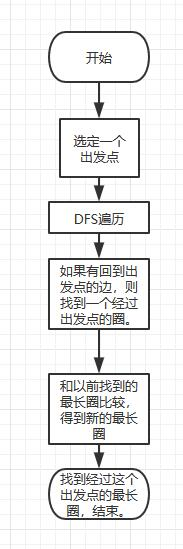
\includegraphics[scale=0.5]{process_4.jpg}
		\caption{无向图中最长圈部分算法流程图}
		\label{process_4}
	\end{figure}

	
	\section{关键代码讲解}
	\subsection{邻接矩阵图类}\par
	\begin{lstlisting}[language=C++,name=邻接矩阵图类]
	// 图类,用邻接矩阵表示无向图
	class MGraph {
		private:
		int* visited = NULL;
		// 从顶k开始由DFS寻找最大圈。
		void FindMaxCircleThrough(int& k, int v, int weight, vector<int>* curCircle);
		public:
		Vertex* vexs = NULL;
		int** arcs = NULL; //邻接矩阵,值直接是权,若为0,则表示不相邻
		bool edgeWeighted = false;
		int vexNum = 0, arcNum = 0;
		vector<int> Articul;
		
		bool hasCircle = false;
		int maxWeight = 0;
		vector<int> maxCircle;
		
		MGraph(string fileName);
		// 打印邻接矩阵
		void PrintMatrix();
		// 找关节点的启动函数,最终找到所有割顶放在Articul中
		void FindArticul();
		// 找割顶的DFS函数
		void DFSArticul(int v0, int& count, int* visited, int* low);
		// 找最大圈的函数
		void FindMaxCircle();
		// 打印最大圈
		void PrintMaxCircle();
		// 打印割顶
		void PrintArticul();
		// 打印可以用于生成Graphviz图的代码()
		void PrintGraphvizCode();
	};
	\end{lstlisting}	
	
	\subsection{邻接表图类}\par
	其中包含弧结点类,顶类,图类。\par
	\begin{lstlisting}[language=C++,name=邻接表图类]
	// 弧结点类。认为弧权均为1,故不设多余信息成员变量
	class ArcNode {
		public:
		int adjVex; // 该弧指向的顶点索引
		ArcNode* nextArc; // 指向下一条弧
		
		ArcNode(int av, ArcNode* na) : adjVex(av), nextArc(na) {};
	};
	
	// 顶类。
	class VNode {
		public:
		int index; // 顶点序号
		ArcNode* firstArc; //第一条邻边
		
		// 默认构造方法
		VNode() : index(-1), firstArc(nullptr) {};
		// 由序号和第一条邻边构造顶
		VNode(int index, ArcNode* fa) : index(index), firstArc(fa) {};
		// 添加一条关联边
		void addAdjArc(ArcNode* arcnode);
	};
	
	class ALGraph {
		public:
		VNode* vexs; //顶
		int vexNum = 0, arcNum = 0; //顶数,边数
		int* distance = NULL; // 由Dijkstra算法得到的最短路径距离
		int* front = NULL; // 由Dijkstra算法得到的前驱结点
		
		// 构造函数:通过文件名构造
		ALGraph(string fileName);
		// Dijkstra算法实现
		void ShortestPath_DIJ();
		// 通过front数组来寻找到0的最短路径
		void printShortestPath(int i);
		// 通过front数组来寻找到0的最短路径
		void printAllShortestPath();
		// 打印邻接表
		void printAdjacentList();
	};
	\end{lstlisting}	
	
	\subsection{寻找关节点代码讲解}\par
	这里值得一说的是:为了用栈来实现,在函数内定义了一个状态类,其中包含v,w,min。其含义与书上递归函数中变量的含义相同。此后只需要用一个状态类栈来完成程序。\par
	\begin{lstlisting}[language=C++, name=寻找关节点代码]
	void MGraph::DFSArticul(int v0, int& count, int* visited, int* low) {
		// 状态类
		class State {
			public:
			int v;
			int w;
			int min;
			State(int v, int w, int min) : v(v), w(w), min(min) {};
		};
		
		stack<State*> DFSStack;
		int w = -1;
		DFSStack.push(new State(v0, w, count+1));
		visited[v0] = ++count;
		
		State* s = DFSStack.top();
		while (!DFSStack.empty()) {
			s = DFSStack.top();
			// 找下一个邻顶(生成树的孩子)
			s->w++;
			while (s->w < vexNum && arcs[s->v][s->w] == 0) s->w++;
			if (s->w >= vexNum) {
				// 则说明所有孩子都访问过了,应pop
				// pop前设置好low
				low[s->v] = s->min;
				DFSStack.pop();
				if (DFSStack.empty())
				return;
				delete s;
				// 对前面的结果进行一些处理,更新min值或确认割顶
				s = DFSStack.top();
				if (low[s->w] < s->min) s->min = low[s->w];
				if (low[s->w] >= visited[s->v]) {
					Articul.push_back(s->v);
				}
				continue;
			}
			if (!visited[s->w]) {
				// 如果没被访问过,则访问它
				State* nexts = new State(s->w, -1, -1);
				visited[nexts->v] = nexts->min = ++count;
				DFSStack.push(nexts);
				continue;
			}
			else if (visited[s->w] < s->min) {
				// 否则,尝试修改s->min(如果需要)
				s->min = visited[s->w];
			}
		}
	}
	\end{lstlisting}
	
	\subsection{寻找最短路径代码讲解}\par
	代码运用的是Dijsktra算法,因此只稍作注释,不多加描述。\par
	\begin{lstlisting}[language=C++, name=寻找最短路径代码]
	void ALGraph::ShortestPath_DIJ()
	{
		// 一些初始化
		bool* defined = new bool[vexNum];
		for (int i = 0; i < vexNum; i++) {
			distance[i] = INT_MAX;
			defined[i] = false;
		}
		// 先考虑0顶
		int v = 0;
		ArcNode* an = vexs[v].firstArc;
		while (an != NULL) {
			distance[an->adjVex] = 1;
			front[an->adjVex] = v;
			an = an->nextArc;
		}
		// 遍历所有顶
		for (int i = 0; i < vexNum; i++) {
			int minD = INT_MAX;
			// 找最短路径顶
			for (int j = 0; j < vexNum; j++) {
				if (!defined[j]) {
					if (distance[j] < minD) {
						v = j; minD = distance[j];
					}
				}
			}
			defined[v] = true;
			// 更新最短路径
			an = vexs[v].firstArc;
			while (an != NULL) {
				if (distance[an->adjVex] > minD + 1) {
					distance[an->adjVex] = minD + 1;
					front[an->adjVex] = v;
				}
				an = an->nextArc;
			}
		}
	}
	\end{lstlisting}
	
	\subsection{输出无向图的Graphviz代码讲解}\par
	代码内容只是对图的连接情况作一个格式化的输出,没有什么不易理解的点,注释如下:\par
	\begin{lstlisting}[language=C++, name=输出无向图的Graphviz代码]
	void MGraph::PrintGraphvizCode() {
		if (!edgeWeighted) {
			// 非带权图
			cout << "graph g {" << endl;
				for (int i = 0; i < vexNum; i++) {
					for (int j = i; j < vexNum; j++) {
						if (arcs[i][j] != 0) {
							cout << "\t" << i << "--" << j << endl;
						}
					}
				}
				cout << "}" << endl;
		}
		else {
			// 带权图
			cout << "graph g {" << endl;
				for (int i = 0; i < vexNum; i++) {
					int a1 = -1;
					int a2 = -1;
					for (int k = 0; k < maxCircle.size(); k++) {
						// 确定k是否是最大圈路径上的顶,如果是,用a1,a2记录其邻顶。
						if (maxCircle[k] == i) {
							a1 = k == maxCircle.size() - 1 ? maxCircle[0] : maxCircle[k + 1];
							a2 = k == 0 ? maxCircle[maxCircle.size() - 1] : maxCircle[k - 1];
							break;
						}
					}
					for (int j = i; j < vexNum; j++) {
						if (arcs[i][j] != 0) {
							// 带颜色考虑的输出
							cout << "\t" << i << "--" << j
							<< "[label = \"" << arcs[i][j] << "\""
							<< ", color = \"" << (j == a1 || j == a2 ? "red" : "black") << "\"]" << endl;
						}
					}
				}
				cout << "}" << endl;;
		}
	}
	\end{lstlisting}
	
	\subsection{无向图中最长圈代码讲解}\par
	实际使用时,对每个顶都是用一次下述函数。\par
	\begin{lstlisting}[language=C++, name=无向图中最长圈代码]
	void MGraph::FindMaxCircleThrough(int& k, int v, int weight, vector<int>* curCircle) {
		visited[v] = true;
		curCircle->push_back(v);
		for (int i = 0; i < vexNum; i++) {
			if (arcs[v][i] != 0) {
				if (i == k && curCircle->size() > 2) {
					//说明找到了一个圈
					if (weight + arcs[v][i] > maxWeight) {
						// 比之前找到的更长
						maxWeight = weight + arcs[v][i];
						maxCircle = *curCircle;
						continue;
					}
				}
				else if (!visited[i]) {
					// 未访问顶,则继续遍历
					FindMaxCircleThrough(k, i, weight + arcs[v][i], curCircle);
					continue;
				}
			}
		}
		curCircle->pop_back();
		visited[v] = false;
	}
	\end{lstlisting}
	
	
	\section{调试分析}
	\subsection{寻找关节点}
	\subsubsection{问题发现与解决}\par
	编写代码的时候,发现并不那么容易用栈来实现这样一个函数。因此最后无可奈何地创建了一个状态类来表示状态,进而使得整个代码和递归极其相似。\par
	\subsubsection{算法的时空复杂度分析}\par
	由于采用邻接矩阵,故空间复杂度几乎为$o(v^{2})$\par
	时间复杂度上,由于只是进行了一次深度优先搜索,由于查找下一个结点需要o(n),而类似递归需要o(n),综合起来应该为$o(n^{2})$\par
	
	\subsection{寻找最短路径}
	\subsubsection{问题发现与解决}
	在这个代码中,由于使用的是Dijkstra算法,原理上比较清晰,没有什么大问题。\par
	\subsubsection{算法的时间复杂度分析}\par
	Dijkstra算法中,每次为了确定一个顶来寻找有最小路径的顶用了o(n),此外,对所有顶都要执行一次这样的操作,因此时间复杂度应该为$o(n^{2})$。\par
	
	\subsection{无向图中的最长圈}
	\subsubsection{问题发现与解决}\par
	使用深度优先搜索时,应该注意返回之后对visited等数据结构的回溯操作,否则将产生错误。\par
	\subsubsection{算法的时间复杂度分析}\par
	每一次深度优先搜索去寻找圈的时候,都用了$o(n^{2})$的时间复杂度,而对每个顶执行一次深度优先搜索,因此总的时间复杂度是$o(n^{3})$\par
	
	
	
	\section{代码测试}
	\subsection{寻找关节点}
	\subsubsection{输入1:}\par
	\fbox{
		\small
		\parbox{0.8\linewidth}{
			8\\
			0 1\\
			0 2\\
			1 2\\
			1 3\\
			1 6\\
			2 5\\
			3 4\\
			3 6\\
			5 6\\
			5 7\\
		}
	}\par
	\textbf{输出截图1:}\par
	\begin{figure}[H]
		\begin{minipage}[H]{0.48\linewidth}
			\centering
			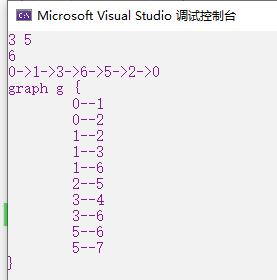
\includegraphics[scale=0.45]{output11.jpg}
			\label{output11}
		\end{minipage}
		\qquad
		\begin{minipage}[H]{0.48\linewidth}
			\centering
			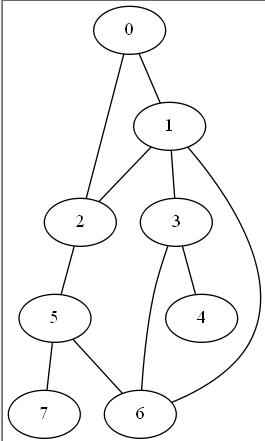
\includegraphics[scale=0.45]{output111.jpg}
			\label{output111}
		\end{minipage}
	\end{figure}
	\subsubsection{输入2:}\par
	\fbox{
		\small
		\parbox{0.8\linewidth}{
			10\\
			0 4\\
			0 9\\
			1 2\\
			1 3\\
			1 4\\
			2 4\\
			2 6\\
			3 5\\
			5 6\\
			5 9\\
			6 7\\
			7 8\\
		}
	}\par
	\textbf{输出截图2:}\par
	\begin{figure}[H]
		\begin{minipage}[H]{0.48\linewidth}
			\centering
			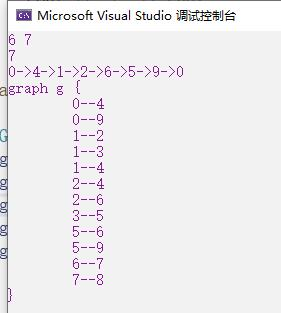
\includegraphics[scale=0.45]{output12.jpg}
			\label{output12}
		\end{minipage}
		\qquad
		\begin{minipage}[H]{0.48\linewidth}
			\centering
			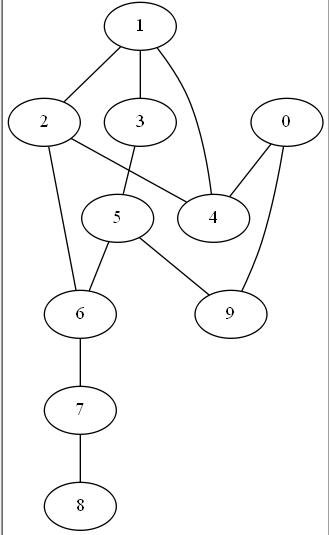
\includegraphics[scale=0.45]{output121.jpg}
			\label{output121}
		\end{minipage}
	\end{figure}
	
	\subsection{寻找最短路径}
	\subsubsection{输入1:}\par
	\fbox{
		\small
		\parbox{0.8\linewidth}{
			8\\
			0 1\\
			0 2\\
			1 2\\
			1 3\\
			1 6\\
			2 5\\
			3 4\\
			3 6\\
			5 6\\
			5 7\\
		}
	}\par
	\textbf{输出截图1:}\par
	\begin{figure}[H]
		\centering
		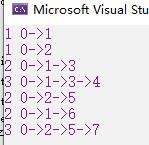
\includegraphics[scale=1]{output21.jpg}
		\label{output21}
	\end{figure}\par
	\subsubsection{输入2:}\par
	\fbox{
		\small
		\parbox{0.8\linewidth}{
			10\\
			0 4\\
			0 9\\
			1 2\\
			1 3\\
			1 4\\
			2 4\\
			2 6\\
			3 5\\
			5 6\\
			5 9\\
			6 7\\
			7 8\\
		}
	}\par
	\textbf{输出截图2:}\par
	\begin{figure}[H]
		\centering
		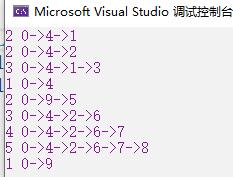
\includegraphics[scale=1]{output22.jpg}
		\label{output22}
	\end{figure}\par
	
	
	
	\subsection{无向图中的最长圈}
	\subsubsection{输入1:}\par
	\fbox{
		\small
		\parbox{0.8\linewidth}{
			10\\
			0 4 2\\
			0 9 1\\
			1 2 6\\
			1 3 3\\
			1 4 9\\
			2 4 5\\
			2 6 5\\
			3 5 6\\
			5 6 4\\
			5 9 6\\
			6 7 5\\
			7 8 5\\
		}
	}\par
	\textbf{输出截图1:}\par
	\begin{figure}[H]
		\begin{minipage}[H]{0.48\linewidth}
			\centering
			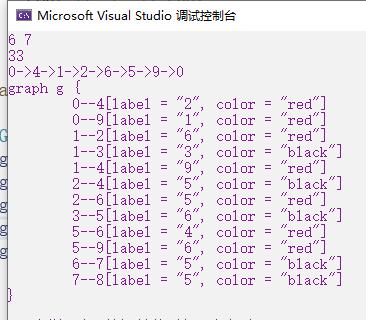
\includegraphics[scale=0.45]{output31.jpg}
			\label{output31}
		\end{minipage}
		\qquad
		\begin{minipage}[H]{0.48\linewidth}
			\centering
			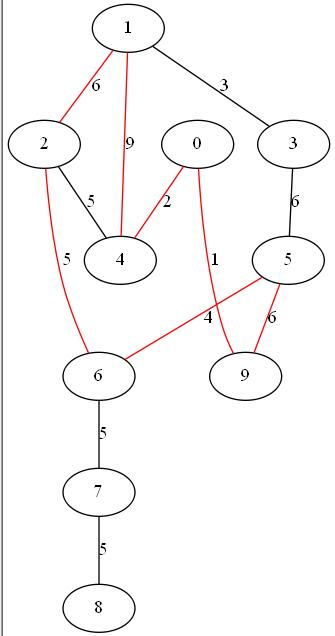
\includegraphics[scale=0.45]{output311.jpg}
			\label{output311}
		\end{minipage}
	\end{figure}
	\subsubsection{输入2:}\par
	\fbox{
		\small
		\parbox{0.8\linewidth}{
			8\\
			0 1 2\\
			0 2 1\\
			1 2 6\\
			1 3 3\\
			1 6 9\\
			2 5 5\\
			3 4 6\\
			3 6 2\\
			5 6 4\\
			5 7 6\\
		}
	}\par
	\textbf{输出截图2:}\par
	\begin{figure}[H]
		\begin{minipage}[H]{0.48\linewidth}
			\centering
			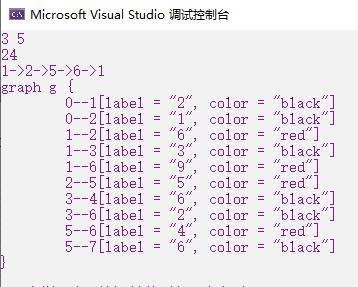
\includegraphics[scale=0.45]{output32.jpg}
			\label{output32}
		\end{minipage}
		\qquad
		\begin{minipage}[H]{0.48\linewidth}
			\centering
			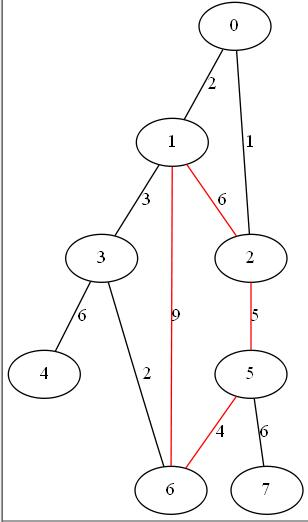
\includegraphics[scale=0.45]{output321.jpg}
			\label{output321}
		\end{minipage}
	\end{figure}
	

	\section{实验总结}
	本次实验中,主要运用了邻接矩阵表示图和邻接表表示图。通过实验可以发现,邻接矩阵便于查找边权关系,而使用邻接表图时,可以方便地查找下一个邻边,以较好地完成遍历操作。另外,图论中的各种定理也比较丰富,应该尽快熟悉各大常用定理,并熟练编写其程序。\par

	
	\section{附录}
	\subsection{附录A.关节点寻找、最长圈寻找及Graphviz代码的输出程序}
	\begin{lstlisting}[language=C++, name=关节点寻找、最长圈寻找及Graphviz代码的输出程序]
	// PB18111697_王章瀚_4_AdjacentMatrix.cpp : 此文件包含 "main" 函数。程序执行将在此处开始并结束。
	//
	
	#include <iostream>
	#include <fstream>
	#include <sstream>
	#include <string>
	#include <climits>
	#include <vector>
	#include <stack>
	#include <algorithm>
	
	using namespace std;
	
	class Vertex {
		public:
		int index;
	};
	
	// 图类,用邻接矩阵表示无向图
	class MGraph {
		private:
		int* visited = NULL;
		// 从顶k开始由DFS寻找最大圈。
		void FindMaxCircleThrough(int& k, int v, int weight, vector<int>* curCircle);
		public:
		Vertex* vexs = NULL;
		int** arcs = NULL; //邻接矩阵,值直接是权,若为0,则表示不相邻
		bool edgeWeighted = false;
		int vexNum = 0, arcNum = 0;
		vector<int> Articul;
		
		bool hasCircle = false;
		int maxWeight = 0;
		vector<int> maxCircle;
		
		MGraph(string fileName);
		// 打印邻接矩阵
		void PrintMatrix();
		// 找关节点的启动函数,最终找到所有割顶放在Articul中
		void FindArticul();
		// 找割顶的DFS函数
		void DFSArticul(int v0, int& count, int* visited, int* low);
		// 找最大圈的函数
		void FindMaxCircle();
		// 打印最大圈
		void PrintMaxCircle();
		// 打印割顶
		void PrintArticul();
		// 打印可以用于生成Graphviz图的代码()
		void PrintGraphvizCode();
	};
	
	void MGraph::FindMaxCircleThrough(int& k, int v, int weight, vector<int>* curCircle) {
		visited[v] = true;
		curCircle->push_back(v);
		for (int i = 0; i < vexNum; i++) {
			if (arcs[v][i] != 0) {
				if (i == k && curCircle->size() > 2) {
					//说明找到了一个圈
					if (weight + arcs[v][i] > maxWeight) {
						// 比之前找到的更长
						maxWeight = weight + arcs[v][i];
						maxCircle = *curCircle;
						continue;
					}
				}
				else if (!visited[i]) {
					// 未访问顶,则继续遍历
					FindMaxCircleThrough(k, i, weight + arcs[v][i], curCircle);
					continue;
				}
			}
		}
		curCircle->pop_back();
		visited[v] = false;
	}
	
	MGraph::MGraph(string fileName) {
		fstream fs(fileName, ios::in | ios::out);
		// 读入顶点数
		string line;
		fs >> vexNum;
		getline(fs, line);
		// 分配顶点的空间
		vexs = new Vertex[vexNum];
		if (vexs == NULL) return;
		for (int i = 0; i < vexNum; i++) {
			vexs[i].index = i;
		}
		// 分配visited的空间
		visited = new int[vexNum];
		if (visited == NULL) return;
		memset(visited, 0, sizeof(int) * vexNum);
		// 分配边矩阵空间
		arcs = new int* [vexNum];
		if (arcs == NULL) return;
		for (int i = 0; i < vexNum; i++) {
			arcs[i] = new int[vexNum];
			if (arcs[i] == NULL) return;
			memset(arcs[i], 0, sizeof(int)*vexNum);
		}
		// 读入数据
		while(!fs.eof()) {
			getline(fs, line);
			stringstream ss(line);
			int h, t;
			ss >> h >> t;
			// 看该行是否有第三个数,如果有说明输入了边权
			if (ss.eof()) {
				arcs[h][t] = 1;
				arcs[t][h] = 1;
			}
			else {
				edgeWeighted = true;
				ss >> arcs[h][t];
				arcs[t][h] = arcs[h][t];
			}
			arcNum++;
		}
		if (arcNum >= vexNum) hasCircle = true;
	}
	
	void MGraph::PrintMatrix() {
		for (int i = 0; i < vexNum; i++) {
			for (int j = 0; j < vexNum; j++) {
				cout << arcs[i][j] << ' ';
			}
			cout << endl;
		}
		cout << endl;
	}
	// 这里假设图连通
	void MGraph::FindArticul() {
		// 全局计数
		int count = 1;
		// 定义访问过标记数组
		int* visited = new int[vexNum];
		if (visited == NULL) return;
		memset(visited, 0, sizeof(int) * vexNum);
		// 定义low数组
		int* low = new int[vexNum];
		if (low == NULL) return;
		memset(low, 0, sizeof(int) * vexNum);
		
		// 第一个结点vexs[0]已经访问
		visited[0] = 1;
		int v = -1;
		while (arcs[0][++v] == 0);
		DFSArticul(v, count, visited, low);
		if (count < vexNum) {
			// 说明生成树中至少有两棵子树,这时根vexs[0]是割顶
			Articul.push_back(0);
			// 继续访问其他子树
			v++;
			while (v < vexNum && arcs[0][v] == 0) v++;
			DFSArticul(v, count, visited, low);
		}
		// 对割顶进行排序
		sort(Articul.begin(), Articul.end(), less<int>());
	}
	
	void MGraph::DFSArticul(int v0, int& count, int* visited, int* low) {
		// 状态类
		class State {
			public:
			int v;
			int w;
			int min;
			State(int v, int w, int min) : v(v), w(w), min(min) {};
		};
		
		stack<State*> DFSStack;
		int w = -1;
		DFSStack.push(new State(v0, w, count+1));
		visited[v0] = ++count;
		
		State* s = DFSStack.top();
		while (!DFSStack.empty()) {
			s = DFSStack.top();
			// 找下一个邻顶(生成树的孩子)
			s->w++;
			while (s->w < vexNum && arcs[s->v][s->w] == 0) s->w++;
			if (s->w >= vexNum) {
				// 则说明所有孩子都访问过了,应pop
				// pop前设置好low
				low[s->v] = s->min;
				DFSStack.pop();
				if (DFSStack.empty())
				return;
				delete s;
				// 对前面的结果进行一些处理,更新min值或确认割顶
				s = DFSStack.top();
				if (low[s->w] < s->min) s->min = low[s->w];
				if (low[s->w] >= visited[s->v]) {
					bool isIn = false;
					for (auto a : Articul) {
						if (a == s->v) {
							isIn = true;
							break;
						}
					}
					if(!isIn) Articul.push_back(s->v);
				}
				continue;
			}
			if (!visited[s->w]) {
				// 如果没被访问过,则访问它
				State* nexts = new State(s->w, -1, -1);
				visited[nexts->v] = nexts->min = ++count;
				DFSStack.push(nexts);
				continue;
			}
			else if (visited[s->w] < s->min) {
				// 否则,尝试修改s->min(如果需要)
				s->min = visited[s->w];
			}
			
		}
		
	}
	
	void MGraph::FindMaxCircle() {
		for (int k = 0; k < vexNum; k++) {
			memset(visited, 0, sizeof(int) * vexNum);
			FindMaxCircleThrough(k, k, 0, new vector<int>);
		}
	}
	
	void MGraph::PrintMaxCircle()
	{
		if (hasCircle) {
			cout << maxWeight << endl << maxCircle[0];
			int vsize = maxCircle.size();
			for (int i = 1; i < vsize; i++) {
				cout << "->" << maxCircle[i];
			}
			cout << "->" << maxCircle[0] << endl;
		}
		else {
			cout << "没有圈" << endl;
		}
	}
	
	void MGraph::PrintArticul() {
		for (auto e : Articul) {
			cout << e << ' ';
		}
		cout << endl;
	}
	
	void MGraph::PrintGraphvizCode() {
		if (!edgeWeighted) {
			// 非带权图
			cout << "graph g {" << endl;
				for (int i = 0; i < vexNum; i++) {
					for (int j = i; j < vexNum; j++) {
						if (arcs[i][j] != 0) {
							cout << "\t" << i << "--" << j << endl;
						}
					}
				}
				cout << "}" << endl;
		}
		else {
			// 带权图
			cout << "graph g {" << endl;
				for (int i = 0; i < vexNum; i++) {
					int a1 = -1;
					int a2 = -1;
					for (int k = 0; k < maxCircle.size(); k++) {
						// 确定k是否是最大圈路径上的顶,如果是,用a1,a2记录其邻顶。
						if (maxCircle[k] == i) {
							a1 = k == maxCircle.size() - 1 ? maxCircle[0] : maxCircle[k + 1];
							a2 = k == 0 ? maxCircle[maxCircle.size() - 1] : maxCircle[k - 1];
							break;
						}
					}
					for (int j = i; j < vexNum; j++) {
						if (arcs[i][j] != 0) {
							// 带颜色考虑的输出
							cout << "\t" << i << "--" << j
							<< "[label = \"" << arcs[i][j] << "\""
							<< ", color = \"" << (j == a1 || j == a2 ? "red" : "black") << "\"]" << endl;
						}
					}
				}
				cout << "}" << endl;;
		}
	}
	
	int main()
	{
		MGraph mg("optional_input2.txt");
		mg.PrintMatrix();
		mg.FindArticul();
		mg.PrintArticul();
		mg.FindMaxCircle();
		mg.PrintMaxCircle();
		mg.PrintGraphvizCode();
	}
	\end{lstlisting}
	
	\subsection{附录B.最短路径搜寻程序}
	\begin{lstlisting}[language=C++, name=最短路径搜寻程序]
	// PB18111697_王章瀚_4_AdjacentList.cpp : 此文件包含 "main" 函数。程序执行将在此处开始并结束。
	//
	
	#include <iostream>
	#include <fstream>
	#include <sstream>
	#include <list>
	#include <string>
	#include <queue>
	#include <stack>
	
	using namespace std;
	
	// 弧结点类。认为弧权均为1,故不设多余信息成员变量
	class ArcNode {
		public:
		int adjVex; // 该弧指向的顶点索引
		ArcNode* nextArc; // 指向下一条弧
		
		ArcNode(int av, ArcNode* na) : adjVex(av), nextArc(na) {};
	};
	
	// 顶类。
	class VNode {
		public:
		int index; // 顶点序号
		ArcNode* firstArc; //第一条邻边
		
		// 默认构造方法
		VNode() : index(-1), firstArc(nullptr) {};
		// 由序号和第一条邻边构造顶
		VNode(int index, ArcNode* fa) : index(index), firstArc(fa) {};
		// 添加一条关联边
		void addAdjArc(ArcNode* arcnode);
	};
	
	class ALGraph {
		public:
		VNode* vexs; //顶
		int vexNum = 0, arcNum = 0; //顶数,边数
		int* distance = NULL; // 由Dijkstra算法得到的最短路径距离
		int* front = NULL; // 由Dijkstra算法得到的前驱结点
		
		// 构造函数:通过文件名构造
		ALGraph(string fileName);
		// Dijkstra算法实现
		void ShortestPath_DIJ();
		// 通过front数组来寻找到0的最短路径
		void printShortestPath(int i);
		// 通过front数组来寻找到0的最短路径
		void printAllShortestPath();
		// 打印邻接表
		void printAdjacentList();
	};
	
	void VNode::addAdjArc(ArcNode* arcnode)
	{
		if (firstArc == NULL) {
			firstArc = arcnode;
			return;
		}
		ArcNode* p = firstArc;
		while (p->nextArc != NULL) p = p->nextArc;
		p->nextArc = arcnode;
		return;
	}
	
	void ALGraph::ShortestPath_DIJ()
	{
		// 一些初始化
		bool* defined = new bool[vexNum];
		for (int i = 0; i < vexNum; i++) {
			distance[i] = INT_MAX;
			defined[i] = false;
		}
		// 先考虑0顶
		int v = 0;
		ArcNode* an = vexs[v].firstArc;
		while (an != NULL) {
			distance[an->adjVex] = 1;
			front[an->adjVex] = v;
			an = an->nextArc;
		}
		// 遍历所有顶
		for (int i = 0; i < vexNum; i++) {
			int minD = INT_MAX;
			// 找最短路径顶
			for (int j = 0; j < vexNum; j++) {
				if (!defined[j]) {
					if (distance[j] < minD) {
						v = j; minD = distance[j];
					}
				}
			}
			defined[v] = true;
			// 更新最短路径
			an = vexs[v].firstArc;
			while (an != NULL) {
				if (distance[an->adjVex] > minD + 1) {
					distance[an->adjVex] = minD + 1;
					front[an->adjVex] = v;
				}
				an = an->nextArc;
			}
		}
	}
	
	ALGraph::ALGraph(string fileName) {
		fstream fs(fileName, ios::in | ios::out);
		// 读入顶点数
		string line;
		fs >> vexNum;
		getline(fs, line);
		// 分配顶点的空间
		vexs = new VNode[vexNum];
		if (vexs == NULL) return;
		for (int i = 0; i < vexNum; i++) {
			vexs[i].index = i;
		}
		// 分配distance空间
		distance = new int[vexNum];
		if (distance == NULL) return;
		memset(distance, 0, sizeof(int) * vexNum);
		// 分配front空间
		front = new int[vexNum];
		if (front == NULL) return;
		memset(front, 0, sizeof(int) * vexNum);
		
		// 读入数据
		while (!fs.eof()) {
			getline(fs, line);
			stringstream ss(line);
			int h, t;
			ss >> h >> t;
			vexs[h].addAdjArc(new ArcNode(t, nullptr));
			vexs[t].addAdjArc(new ArcNode(h, nullptr));
			arcNum++;
		}
	}
	
	void ALGraph::printShortestPath(int i)
	{
		int t = i;
		stack<int> s;
		while (t != 0) {
			s.push(t);
			t = front[t];
		}
		int ssize = s.size();
		cout << distance[i] << " 0";
		for (int t = 0; t < ssize; t++) {
			cout << "->" << s.top();
			s.pop();
		}
		cout << endl;
	}
	
	void ALGraph::printAllShortestPath()
	{
		for (int i = 1; i < vexNum; i++) {
			printShortestPath(i);
		}
	}
	
	void ALGraph::printAdjacentList()
	{
		for (int i = 0; i < vexNum; i++) {
			cout << i << ":";
			ArcNode* p = vexs[i].firstArc;
			while (p != NULL) {
				cout << p->adjVex << " ";
				p = p->nextArc;
			}
			cout << endl;
		}
	}
	
	
	
	int main()
	{
		ALGraph alg("input2.txt");
		alg.ShortestPath_DIJ();
		alg.printAllShortestPath();
	}
	\end{lstlisting}
	
\end{document}
